\section{The Virtual KITTI 3D Dataset}
\label{sec:dataset}

For their experiments, the authors decided to use the large \gls{lidar} point cloud dataset of the urban area of Ottawa. This large dataset allowed the authors to balanced the samples used for training: the idea is to have the same amount of samples for each label. We needed to find a dataset large enough and interesting enough to be adequate.\\

We finally decided to use the Virtual KITTI 3D Dataset for Semantic Segmentation. More information about it can be found \href{https://github.com/VisualComputingInstitute/vkitti3D-dataset.git}{here}. This dataset contains labelled point clouds of vehicles surroundings. We decided to use this dataset for 4 main reasons.
\begin{itemize}
    \item[\(\bullet \)] It is simple to use, we created scripts to exploit and visualize it easily.
    \item[\(\bullet \)] It is an interesting dataset since it can directly be related to the actual autonomous vehicle challenge.
    \item[\(\bullet \)] It is a more complex dataset since there are 13 possible classes (compare to 7 for the one useb by the authors) and it is then more complicated to balance the samples.
    \item[\(\bullet \)] It looks nice, as you can see in the figures \ref{pic1} and \ref{pic2}.
\end{itemize}

\begin{figure}[H]
    \centering
	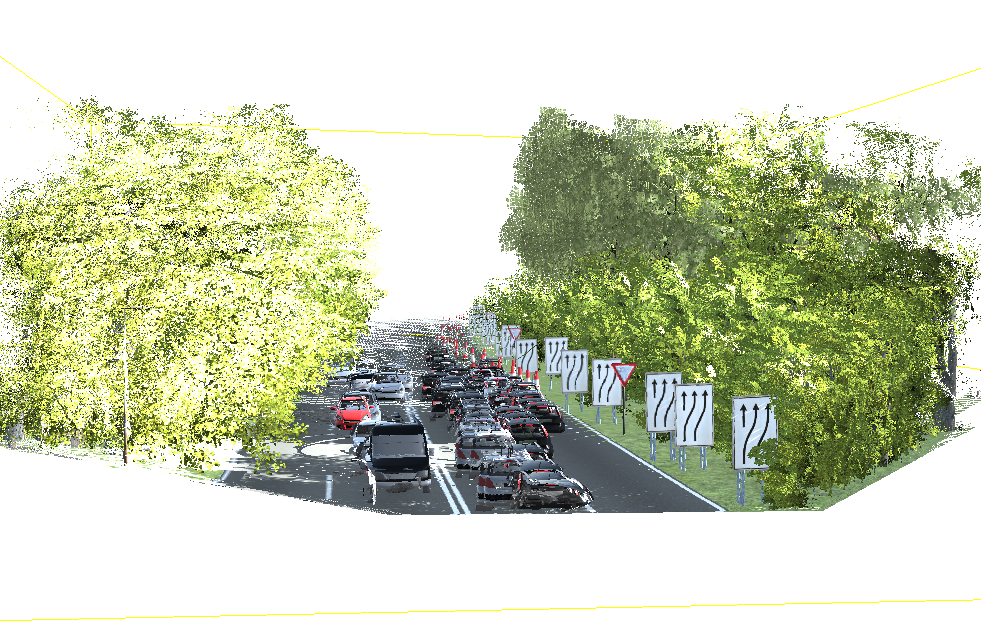
\includegraphics[scale=0.3]{sources/pic1.png}
	\caption{Point cloud colorized}
	\label{pic1}
\end{figure}

\begin{figure}[H]
    \centering
	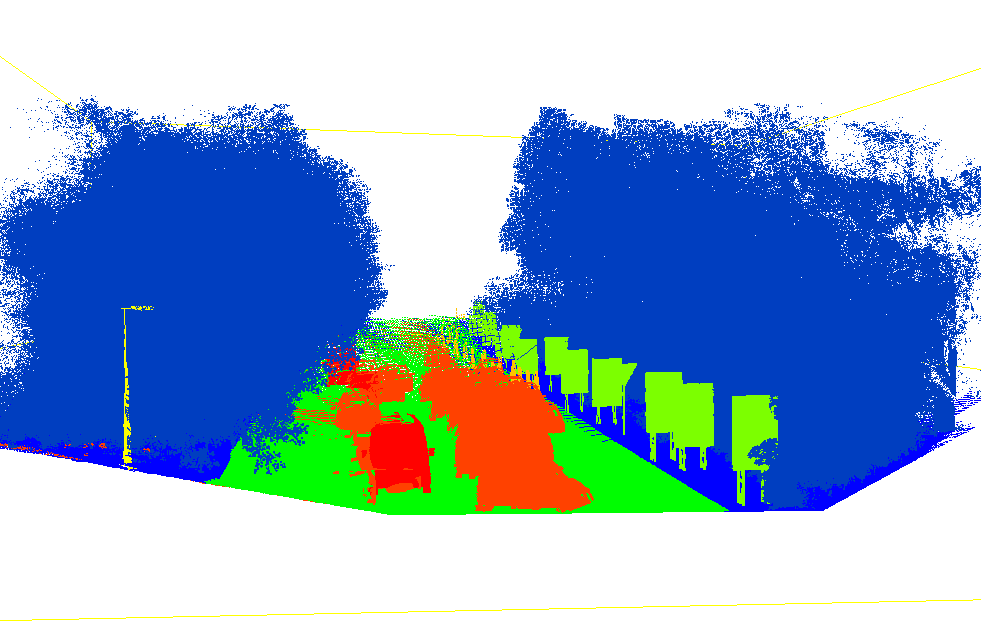
\includegraphics[scale=0.3]{sources/pic2.png}
	\caption{Point cloud labelized}
	\label{pic2}
\end{figure}
